% !TEX encoding = UTF-8 Unicode
\documentclass[a4paper]{article}

\usepackage{url}

\usepackage{graphicx}
\graphicspath{{../slike}}

\begin{document}

\title{Intrinsically disordered proteins (\textit{IDPs}) in \textit{SARS-CoV-2} interactome {\large (manuscript)}}

\author{Lazar Vasović {\small (student)}\\Gordana Pavlović-Lažetić {\small (professor)}}

\maketitle

\abstract{This manuscript discusses the properties of proteins and their relations in the interactomes of the selected subsets of \textit{SARS-CoV-2} proteome -- membrane, non-structural proteins, and, finally, full proteome. Protein disorder and respective node degrees in the protein interaction networks were singled out as the features of interest. Viral interactomes were also combined with that of human lung tissue so as to establish which connections in the resulting viral-host interactome are interesting and how they are linked to protein disorder. Results, which include several scatter plots and correlation analysis, indicate that hubs (highly connected nodes) and their neighbors tend to be on average more ordered than proteins with a small number of connections and their neighbors. This is in contrast to the similar studies conducted on eukaryotic interactomes and possibly opens the path to a new direction of research on viral interactomes.}

\tableofcontents

\newpage

\section{Introduction}
\label{intro}

\textbf{Biological systems} are typically viewed as networks of mutually interacting \textbf{basic building blocks} \cite{junker, guzzi}. Units that operate independently are rare, so \textbf{interactions} are a key part of any biological system. In fact, no system can be viewed as a simple sum of elements. This is true both for small cells and huge ecosystems, and the only significant difference between them is the type of basic blocks. Example microblocks (small basic blocks) are genes, proteins, and metabolites, while individual organisms and generally species are considered macroblocks (big basic blocks).

In order to conduct \textbf{computational analysis} of biological systems, it is necessary to choose an appropriate \textbf{mathematical model}. One natural model of interacting blocks is a \textbf{graph}. The use of graph formalism enables the effective representation of the real-life entities and the complex and mutual interrelationships among those entities. Basic blocks are represented as graph \textbf{nodes} and interactions as graph \textbf{edges}. Of course, this representation has its flaws, mostly because it oversimplifies some complex non-binary interactions. However, it is still quite a useful abstraction, since it opens the path to effective computational analysis.

\textbf{Protein interaction networks (\textit{PINs})}, also known as protein-protein interaction networks (\textit{PPINs} or \textit{PPI} networks), are an important class of biological systems. Each their node represents a \textbf{protein}, while \textbf{undirected} edges encapsulate binary physical interaction between two proteins, also known as \textbf{protein-protein interactions (\textit{PPIs})}. As a part of larger \textit{omics} studies, \textit{PINs} are also known as \textbf{interactomes} and graph nodes as \textbf{interactors}. The importance of these networks lies in the fact that protein molecules are the workhorses of the cell, performing and controlling almost all activities in an organism. For example, highly connected proteins (hubs) within a network are most probably vital molecules and are in many cases more essential for survival than proteins with lower connectivity. Related \textit{PINs} can also be aligned with each other as a way of identifying substructures that have been preserved throughout evolution. Densely connected parts of the network may represent potential protein complexes, which is an additional benefit of using graph formalism.

One particularly interesting class of proteins are \textbf{intrinsically disordered proteins (\textit{IDPs})}. These proteins lack a fixed and well-defined three-dimensional structure and are highly abundant in nature \cite{uversky}. Their conformational flexibility (intrinsic disorder) may be present in a molten globular form, in a form of a random coil, or a pre-molten globule. Only a few proteins are fully disordered in their native state, so \textit{IDPs} also include semi-disordered proteins, whose flexible parts are called \textbf{intrinsically disordered regions (\textit{IDRs})}. \textit{IDPs} and \textit{IDRs} often facilitate protein-protein interactions, being flexible linkers and binding to multiple partners, thus \textit{IDPs} frequently serve as hubs in complex \textit{PPI} networks.

In the last years, many authors have researched the topic of interactomics and intrinsically disordered proteins. Much has been revealed about the biological importance of \textit{IDPs}/\textit{IDRs}, as well as their \textbf{markedly big} interactomes \cite{teilum, cumberworth}. Most studies in the field of bioinformatics and computational analysis focused on exploring \textit{PINs} of eukaryotic organisms such as human (\textit{Homo sapiens}) and baker's yeast (\textit{Saccharomyces cerevisiae}). There is an agreement between these papers that hubs, which are highly connected nodes, are \textbf{on average more disordered} than ends, which are proteins with a small number of connections \cite{haynes, dosztanyi, singh, patil, hu}.

Contrary to the related work, this manuscript focuses on analyzing the interactomes of the selected subsets of \textbf{\textit{SARS-CoV-2} proteome}. \textit{SARS-CoV-2} is a virus, so its proteins could possibly act differently than those of eukaryotes. Protein \textbf{disorder degree} and respective \textbf{node degrees} in the \textit{PINs} were singled out as the features of interest. Additionally, since merged \textbf{viral-host interactomes} had been found as useful in establishing which interactions are biologically interesting \cite{gao}, viral interactomes were combined with that of human lung tissue. This made it possible to discuss if links in the viral-host interplay are related to protein disorder. The methodology is described in section \ref{meth}, while results, which are based on several scatter plots and correlation analysis, are shown in section \ref{res}.

\section{Materials and methods}
\label{meth}

The paper aimed to examine several \textit{SARS-CoV-2} interactomes, all constructed from \textbf{publicly available data}. Four different graphs were chosen as the starting point, with their core properties shown in table \ref{inter}.

\begin{table}[h!]
  \centering
  \caption{Analyzed interactomes and their properties}
  \resizebox{.9\textwidth}{!}{%
  \begin{tabular}{c | c c | c c}
     & Main protein(s) & Source database & Nodes & Edges \\ \hline
    M\_IntAct & membrane (M) & IntAct & 198 & 294 \\
    M\_iRef & membrane (M) & iRefIndex & 211 & 451 \\
    Nsp\_iRef & non-structural (NSPs) & iRefIndex & 311 & 1066 \\
    SARS2\_iRef & full proteome & iRefIndex & 1419 & 8722 \\
  \end{tabular}}
  \label{inter}
\end{table}

As an example, the interactome of non-structural proteins (\textit{NSPs}) is shown in figure \ref{nsp}. Nodes are \textbf{colored} by origin -- human are blue, while viral are orange. Node \textbf{size} is proportional to its degree in the network.

\begin{figure}[h!]
  \centering
  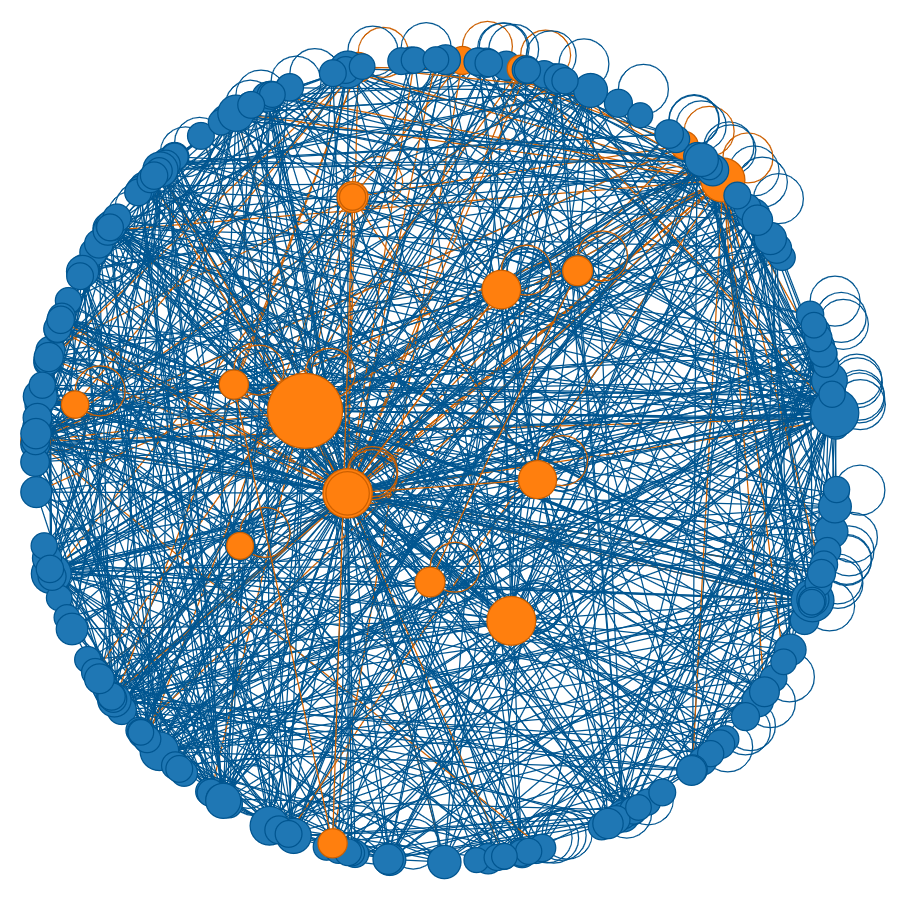
\includegraphics[scale=0.45]{Nsp_iRef.png}
  \caption{Nsp\_iRef, interactome of non-structural proteins}
  \label{nsp}
\end{figure}

Database \textbf{\textit{IntAct}}\footnotemark \footnotetext{IntAct Molecular Interaction Database: \url{https://www.ebi.ac.uk/intact/home}} was initially chosen as one of the most popular in the field of protein-protein interaction warehousing. It, however, doesn't include separate data for the \textit{NSPs} of the considered \textit{SARS-CoV-2}\footnotemark\footnotetext{SARS-CoV-2: \url{https://www.ncbi.nlm.nih.gov/Structure/SARS-CoV-2.html}}, which makes it inappropriate for conducting full-scale analysis. Instead, \textbf{\textit{iRefIndex}}\footnotemark \footnotetext{iRefIndex PSICQUIC WS: \url{https://irefindex.vib.be/}} was chosen as the only significant database that meets the coverage criterion. Both databases were queried by protein \textit{IDs} and the resulting lists of \textit{PPIs} were used for building the networks. It can be noted that \textit{iRefIndex} produces \textbf{noticeably denser} networks in comparison to \textit{IntAct}, i.e. it contains many additional interactions. Another interesting fact is that the graphs containing non-structural proteins (\textit{Nsp} and \textit{SARS2\_iRef}) are much \textbf{more connected} than those without them (\textit{M}).

Two additional interactomes were taken into consideration so as to analyze the dynamics of viral-host interplay. They are shown in table \ref{addit}.

\begin{table}[h!]
  \centering
  \caption{Additional interactomes and their properties}
  \resizebox{.9\textwidth}{!}{%
  \begin{tabular}{c | c c | c c}
     & Main proteins & Source database & Nodes & Edges \\ \hline
    SARS\_iRef & only viral proteins & iRefIndex & 30 & 42 \\
    lungs\_HuRI & human lung tissue & NDEx & 175 & 162 \\
  \end{tabular}}
  \label{addit}
\end{table}

The first graph, containing only \textbf{viral proteins}, is shown in figure \ref{viral}.

\begin{figure}[h!]
  \centering
  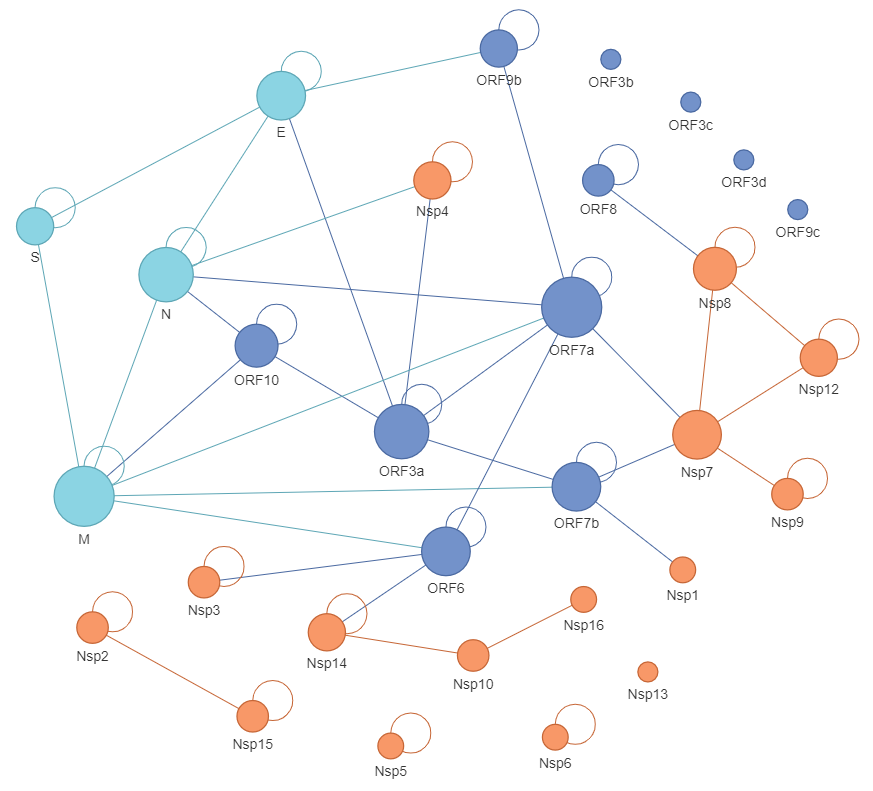
\includegraphics[scale=0.55]{SARS_iRef.png}
  \caption{SARS\_iRef, interactome with only viral proteins}
  \label{viral}
\end{figure}

Nodes are colored by their type. Light blue denotes structural proteins, which are spike (\textit{S}), envelope (\textit{E}), membrane (\textit{M}), and nucleocapsid (\textit{N}). Orange stands for non-structural proteins, which are \textit{Nsp1} to \textit{Nsp16} (not all are present in \textit{iRefIndex}). Dark blue represents accessory proteins, which are \textit{ORFs}. Once again, size is proportional to node degree.

The second graph, which represents the interactome of the \textbf{human lung tissue}, was taken from a reference map of the human binary protein interactome known as \textbf{\textit{HuRI}} (\textit{Human Reference Interactome}) \cite{luck}. The network itself was downloaded from the \textbf{\textit{NDEx}}\footnotemark \footnotetext{NDEx: \url{https://www.ndexbio.org/#/network/289c6fe3-5fb9-11e9-9f06-0ac135e8bacf}} database. It was chosen because \textit{SARS-CoV-2} is a respiratory virus and is shown in figure \ref{lungs}. It is made of two distinct types of nodes -- hubs (green) and ends (blue).

\begin{figure}[h!]
  \centering
  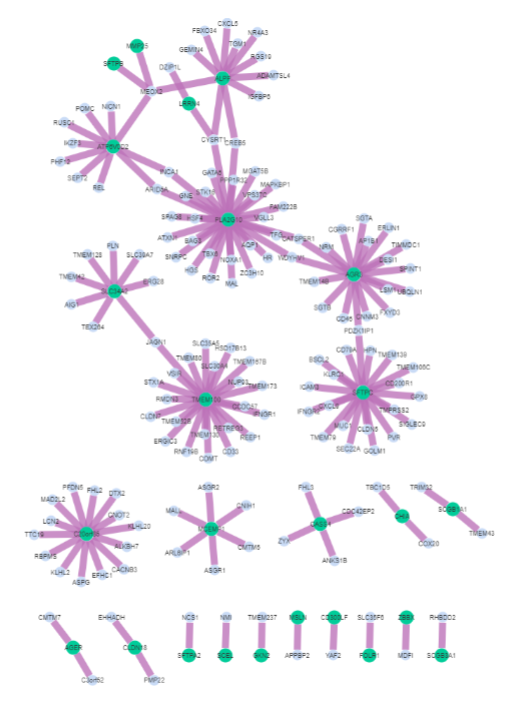
\includegraphics[scale=0.65]{pluca_HuRI.png}
  \caption{lungs\_HuRI, interactome of human lung tissue}
  \label{lungs}
\end{figure}

The additional interactomes were combined and the nature of the links in the merged network was examined. Discussion is given in section \ref{res}.

Since the idea was to analyze the protein disorder in the studied interactomes, the next step was to choose appropriate \textbf{disorder predictors}. Amino acid composition\footnotemark, \footnotetext{Composition Profiler: \url{http://www.cprofiler.org/help.html}} \textit{PONDR}\footnotemark \footnotetext{Predictor of Natural Disordered Regions (PONDR): \url{http://www.pondr.com/}} family, and charge-hydropathy (\textit{CH})\footnotemark[6] were the methods of choice. Number of short (at least five residues in length) and long (more than thirty residues in length) disordered regions, as well as the average disorder of neighbors ("the other side of interactions") were additionally considered. Specialized databases like \textit{DisProt} and \textit{D²P²} lack many \textit{SARS-CoV-2} proteins, so they were disregarded.

\textbf{Correlation analysis} was the main method used. The relationship between node degree and disorder degree of the respective protein and its neighbors according to all the listed predictors was represented on the plane, as a series of \textbf{scatter plots}. Node degree was put on the horizontal axis, while the vertical axis was reserved for the output of disorder predictors. Concrete examples and discussion are given in section \ref{res}, dedicated to the results. The entire processing, which ranges from retrieving the data to the final analyses, was done as a \textbf{\textit{Python}}\footnotemark \footnotetext{Python programming language: \url{https://www.python.org/}} script.

\section{Results}
\label{res}

\newpage
\addcontentsline{toc}{section}{References}
\appendix
\bibliography{IDP_in_SARS-CoV-2} 
\bibliographystyle{unsrt}

\end{document}
